% !LW recipe=latexmk (lualatex)

% Compile from this directory: lualatex -halt-on-error poster.tex
% A3 portrait. Copy, artwork and typography remain separate and editable.
\documentclass{article}
\usepackage[paperwidth=297mm,paperheight=420mm,margin=0mm]{geometry}
\usepackage{fontspec}
\usepackage{graphicx}
\usepackage{xcolor}
\usepackage{tikz}
\usetikzlibrary{calc,fadings}
\usepackage{qrcode}
\usepackage[unicode,pdfencoding=auto,hidelinks]{hyperref}

% These are the same SIL Open Font License fonts bundled with the website.
\setmainfont{stix-two-text-normal-400.ttf}[
  Path=fonts/,
  BoldFont=stix-two-text-normal-600.ttf,
  ItalicFont=stix-two-text-italic-400.ttf,
  Ligatures=TeX
]
\definecolor{Paper}{HTML}{F7F6F2}
\definecolor{Ink}{HTML}{202020}
\definecolor{Muted}{HTML}{52677F}
\definecolor{Teal}{HTML}{176365}
\definecolor{Rule}{HTML}{CDD3DA}
\pagecolor{Paper}
\color{Ink}
\pagestyle{empty}
\setlength{\parindent}{0pt}
\setlength{\parskip}{0pt}
% Editable conference copy. Generated from the website's local data.
% Re-run sync-content.mjs to refresh names, affiliations, dates and venue.
\newcommand{\PosterTitle}{Enumerative Geometry in East Asia}
\newcommand{\PosterTitleFirst}{Enumerative}
\newcommand{\PosterTitleSecond}{Geometry}
\newcommand{\PosterTitleThird}{in East Asia}
\newcommand{\PosterSeries}{EGEA}
\newcommand{\PosterYear}{2026}
\newcommand{\PosterDates}{December 7–11, 2026}
\newcommand{\PosterVenue}{Hong Kong University of Science and Technology}
\newcommand{\PosterRoom}{Cheung On Tak Lecture Theater (LT-E), 1/F Academic Building}
\newcommand{\PosterAddress}{Clear Water Bay, Kowloon, Hong Kong SAR}
\newcommand{\PosterURL}{https://egea-2026.github.io/}
\newcommand{\PosterURLLabel}{egea-2026.github.io}
\newcommand{\PosterFooter}{}

% Read down the left column, then down the right, as on the website.
\newcommand{\PosterSpeakersLeft}{%
  \PosterSpeaker{Christopher Brav}{Shanghai Institute for Mathematics and Interdisciplinary Sciences}%
  \PosterSpeaker{Chenjing Bu}{University of Oxford}%
  \PosterSpeaker{Lucien Hennecart}{Centre National de la Recherche Scientifique}%
  \PosterSpeaker{Adeel Khan}{Academia Sinica}%
  \PosterSpeaker{Tasuki Kinjo}{RIMS (Research Institute for Mathematical Sciences), Kyoto University}%
  \PosterSpeaker{Chunyi Li}{University of Warwick}%
  \PosterSpeaker{Woonam Lim}{Yonsei University}%
  \PosterSpeaker{Alexandre Minets}{University of Bonn}%
  \PosterSpeaker{Andres Ibanez Nunez}{University of Edinburgh}%
}
\newcommand{\PosterSpeakersRight}{%
  \PosterSpeaker{Tudor Padurariu}{University of Bonn}%
  \PosterSpeaker{Hyeonjun Park}{Korea Institute for Advanced Study}%
  \PosterSpeaker{Francesco Sala}{Università di Pisa}%
  \PosterSpeaker{Junliang Shen}{Yale University}%
  \PosterSpeaker{Yukinobu Toda}{Kavli IPMU, University of Tokyo}%
  \PosterSpeaker{Junwu Tu}{ShanghaiTech University}%
  \PosterSpeaker{Qizheng Yin}{BICMR, Peking University}%
  \PosterSpeaker{Yang Zhou}{Shanghai Center for Mathematical Sciences, Fudan University}%
  \PosterSpeaker{Zhengyu Zong}{Department of Mathematical Sciences, Tsinghua University}%
}

\hypersetup{
  pdftitle={\PosterTitle\space \PosterYear},
  pdfauthor={EGEA 2026},
  pdfsubject={Conference poster, A3 portrait},
  pdfkeywords={enumerative geometry, East Asia, HKUST, conference}
}

% A common 18 mm rhythm keeps both columns aligned even when an affiliation
% wraps onto a second line. All lettering is live, embedded-font PDF text.
\newcommand{\PosterSpeaker}[2]{%
  \par\nointerlineskip
  \vbox to 18mm{%
    \hsize=119mm\linewidth=119mm\raggedright
    {\fontsize{18}{21}\selectfont #1\par}%
    \vskip 1.1mm
    {\color{Muted}\fontsize{11.2}{13.1}\selectfont #2\par}%
    \vss
  }%
  \par
}
\newcommand{\Kicker}[1]{{\color{Teal}\fontsize{10.5}{13}\selectfont
  \addfontfeatures{LetterSpace=13}\MakeUppercase{#1}}}

\begin{document}
\null
\begin{tikzpicture}[remember picture,overlay,x=1mm,y=-1mm]
  \begin{scope}[shift={(current page.north west)}]
    % Decorative image layer only. No conference text is baked into the image.
% Website artwork, converted losslessly from public/images/landscape.webp.
% Aspect ratio is preserved. A paper-colored fade joins it to the plain field.
\node[anchor=north west,inner sep=0pt] at (0,0)
  {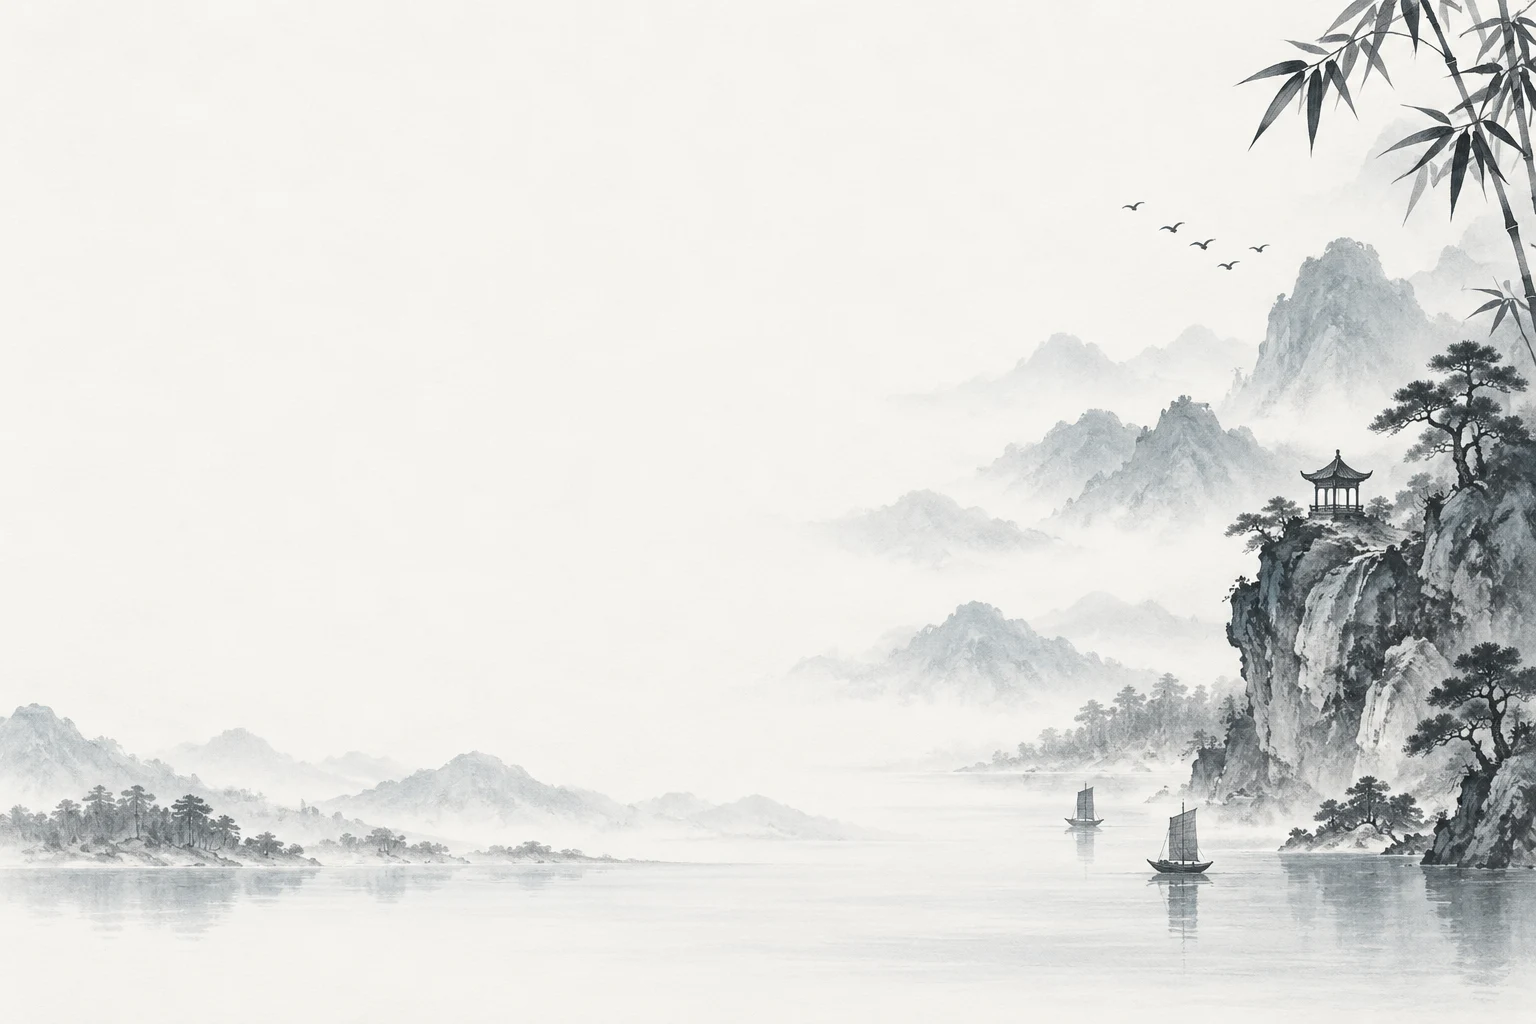
\includegraphics[width=297mm]{assets/landscape.png}};
\fill[Paper,path fading=east] (0,118) rectangle (196,182);
\fill[Paper,path fading=north] (0,179) rectangle (297,198.1);
\fill[Paper] (0,198) rectangle (297,420);


    \node[anchor=north west,inner sep=0pt] at (21,21)
      {\Kicker{\PosterSeries\enspace /\enspace \PosterYear}};

    \node[anchor=north west,inner sep=0pt] at (20,39)
      {\fontsize{65}{65}\selectfont \PosterTitleFirst};
    \node[anchor=north west,inner sep=0pt] at (20,62)
      {\fontsize{65}{65}\selectfont \PosterTitleSecond};
    \node[anchor=north west,inner sep=0pt] at (20,87)
      {\fontsize{55}{61}\selectfont \PosterTitleThird};

    \draw[Teal,line width=.65pt] (21,118) -- (42,118);
    \node[anchor=north west,inner sep=0pt,text=Teal] at (21,125)
      {\fontsize{25}{29}\selectfont \PosterDates};
    \node[anchor=north west,inner sep=0pt,text width=155mm,align=left]
      at (21,141) {\fontsize{17}{20}\selectfont \PosterVenue\par};
    \node[anchor=north west,inner sep=0pt,text width=165mm,align=left]
      at (21,148) {\fontsize{12}{12}\selectfont \PosterRoom\par};
    \node[anchor=north west,inner sep=0pt,text=Muted]
      at (21,159) {\fontsize{11.5}{14}\selectfont \PosterAddress};

    \node[anchor=north west,inner sep=0pt] at (21,195)
      {\Kicker{Invited speakers}};
    \draw[Rule,line width=.5pt] (21,205) -- (276,205);

    \node[anchor=north west,inner sep=0pt,text width=119mm,align=left]
      at (21,214) {\PosterSpeakersLeft};
    \node[anchor=north west,inner sep=0pt,text width=119mm,align=left]
      at (157,214) {\PosterSpeakersRight};

    \draw[Rule,line width=.5pt] (21,382) -- (276,382);
    \node[anchor=north west,inner sep=0pt] at (21,389)
      {\fontsize{16}{19}\selectfont
        \href{\PosterURL}{\PosterURLLabel}};
    \node[anchor=north west,inner sep=0pt,text=Muted] at (21,400)
      {\fontsize{10.5}{13}\selectfont \PosterFooter};
    % The unprinted paper around the code supplies a generous quiet zone.
    \node[anchor=north east,inner sep=0pt,text=Teal] at (273,388)
      {\qrcode[height=18mm,level=M]{\PosterURL}};
  \end{scope}
\end{tikzpicture}
\end{document}
